\chapter{The Carnival at Rome}

When Franz recovered his senses, he saw Albert drinking a glass of
water, of which, to judge from his pallor, he stood in great need; and
the count, who was assuming his masquerade costume. He glanced
mechanically towards the piazza—the scene was wholly changed; scaffold,
executioners, victims, all had disappeared; only the people remained,
full of noise and excitement. The bell of Monte Citorio, which only
sounds on the pope’s decease and the opening of the Carnival, was
ringing a joyous peal.

“Well,” asked he of the count, “what has, then, happened?”

“Nothing,” replied the count; “only, as you see, the Carnival has
commenced. Make haste and dress yourself.”

“In fact,” said Franz, “this horrible scene has passed away like a
dream.”

“It is but a dream, a nightmare, that has disturbed you.”

“Yes, that I have suffered; but the culprit?”

“That is a dream also; only he has remained asleep, while you have
awakened; and who knows which of you is the most fortunate?”

“But Peppino—what has become of him?”

“Peppino is a lad of sense, who, unlike most men, who are happy in
proportion as they are noticed, was delighted to see that the general
attention was directed towards his companion. He profited by this
distraction to slip away among the crowd, without even thanking the
worthy priests who accompanied him. Decidedly man is an ungrateful and
egotistical animal. But dress yourself; see, M. de Morcerf sets you the
example.”

Albert was drawing on the satin pantaloon over his black trousers and
varnished boots.

“Well, Albert,” said Franz, “do you feel much inclined to join the
revels? Come, answer frankly.”

“\textit{Ma foi}, no,” returned Albert. “But I am really glad to have seen
such a sight; and I understand what the count said—that when you have
once habituated yourself to a similar spectacle, it is the only one
that causes you any emotion.”

\begin{figure}[ht]
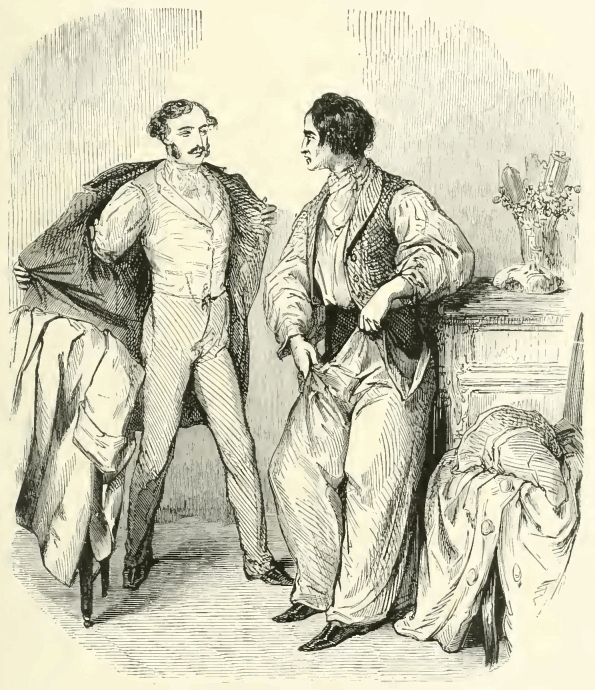
\includegraphics[width=\textwidth]{20175m.jpg}
\end{figure}

“Without reflecting that this is the only moment in which you can study
character,” said the count; “on the steps of the scaffold death tears
off the mask that has been worn through life, and the real visage is
disclosed. It must be allowed that Andrea was not very handsome, the
hideous scoundrel! Come, dress yourselves, gentlemen, dress
yourselves.”

Franz felt it would be ridiculous not to follow his two companions’
example. He assumed his costume, and fastened on the mask that scarcely
equalled the pallor of his own face. Their toilet finished, they
descended; the carriage awaited them at the door, filled with
sweetmeats and bouquets. They fell into the line of carriages.

It is difficult to form an idea of the perfect change that had taken
place. Instead of the spectacle of gloomy and silent death, the Piazza
del Popolo presented a spectacle of gay and noisy mirth and revelry. A
crowd of masks flowed in from all sides, emerging from the doors,
descending from the windows. From every street and every corner drove
carriages filled with clowns, harlequins, dominoes, mummers,
pantomimists, Transteverins, knights, and peasants, screaming,
fighting, gesticulating, throwing eggs filled with flour, confetti,
nosegays, attacking, with their sarcasms and their missiles, friends
and foes, companions and strangers, indiscriminately, and no one took
offence, or did anything but laugh.

Franz and Albert were like men who, to drive away a violent sorrow,
have recourse to wine, and who, as they drink and become intoxicated,
feel a thick veil drawn between the past and the present. They saw, or
rather continued to see, the image of what they had witnessed; but
little by little the general vertigo seized them, and they felt
themselves obliged to take part in the noise and confusion.

A handful of confetti that came from a neighboring carriage, and which,
while it covered Morcerf and his two companions with dust, pricked his
neck and that portion of his face uncovered by his mask like a hundred
pins, incited him to join in the general combat, in which all the masks
around him were engaged. He rose in his turn, and seizing handfuls of
confetti and sweetmeats, with which the carriage was filled, cast them
with all the force and skill he was master of.

\begin{figure}[ht]
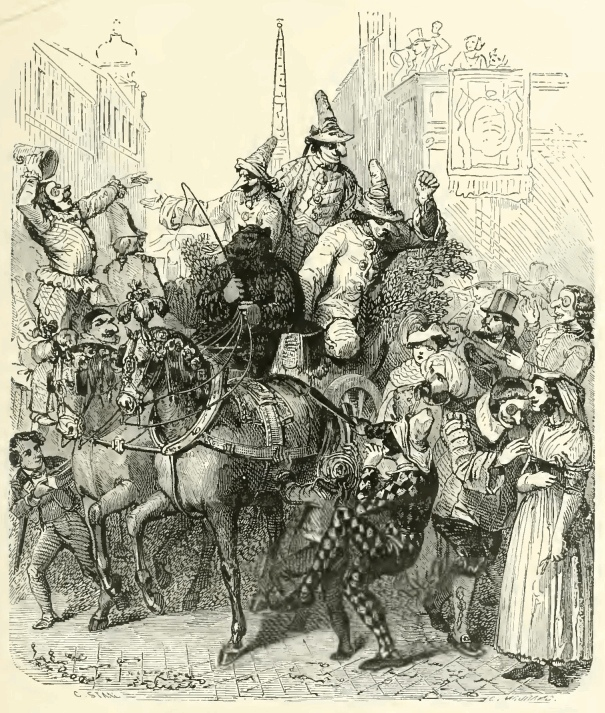
\includegraphics[width=\textwidth]{20177m.jpg}
\end{figure}

The strife had fairly begun, and the recollection of what they had seen
half an hour before was gradually effaced from the young men’s minds,
so much were they occupied by the gay and glittering procession they
now beheld.

As for the Count of Monte Cristo, he had never for an instant shown any
appearance of having been moved. Imagine the large and splendid Corso,
bordered from one end to the other with lofty palaces, with their
balconies hung with carpets, and their windows with flags. At these
balconies are three hundred thousand spectators—Romans, Italians,
strangers from all parts of the world, the united aristocracy of birth,
wealth, and genius. Lovely women, yielding to the influence of the
scene, bend over their balconies, or lean from their windows, and
shower down confetti, which are returned by bouquets; the air seems
darkened with the falling confetti and flying flowers. In the streets
the lively crowd is dressed in the most fantastic costumes—gigantic
cabbages walk gravely about, buffaloes’ heads bellow from men’s
shoulders, dogs walk on their hind legs; in the midst of all this a
mask is lifted, and, as in Callot’s Temptation of St. Anthony, a lovely
face is exhibited, which we would fain follow, but from which we are
separated by troops of fiends. This will give a faint idea of the
Carnival at Rome.

At the second turn, the count stopped the carriage, and requested
permission to withdraw, leaving the vehicle at their disposal. Franz
looked up—they were opposite the Rospoli Palace. At the centre window,
the one hung with white damask with a red cross, was a blue domino,
beneath which Franz’s imagination easily pictured the beautiful Greek
of the Argentina.

“Gentlemen,” said the count, springing out, “when you are tired of
being actors, and wish to become spectators of this scene, you know you
have places at my windows. In the meantime, dispose of my coachman, my
carriage, and my servants.”

We have forgotten to mention, that the count’s coachman was attired in
a bear-skin, exactly resembling Odry’s in \textit{The Bear and the Pasha}; and
the two footmen behind were dressed up as green monkeys, with spring
masks, with which they made grimaces at everyone who passed.

Franz thanked the count for his attention. As for Albert, he was busily
occupied throwing bouquets at a carriage full of Roman peasants that
was passing near him. Unfortunately for him, the line of carriages
moved on again, and while he descended the Piazza del Popolo, the other
ascended towards the Palazzo di Venezia.

“Ah, my dear fellow,” said he to Franz; “you did not see?”

“What?”

“There,—that calash filled with Roman peasants.”

“No.”

“Well, I am convinced they are all charming women.”

“How unfortunate that you were masked, Albert,” said Franz; “here was
an opportunity of making up for past disappointments.”

“Oh,” replied he, half laughing, half serious; “I hope the Carnival
will not pass without some amends in one shape or the other.”

But, in spite of Albert’s hope, the day passed unmarked by any
incident, excepting two or three encounters with the carriage full of
Roman peasants. At one of these encounters, accidentally or purposely,
Albert’s mask fell off. He instantly rose and cast the remainder of the
bouquets into the carriage. Doubtless one of the charming females
Albert had detected beneath their coquettish disguise was touched by
his gallantry; for, as the carriage of the two friends passed her, she
threw a bunch of violets. Albert seized it, and as Franz had no reason
to suppose it was meant for him, he suffered Albert to retain it.
Albert placed it in his button-hole, and the carriage went triumphantly
on.

“Well,” said Franz to him; “there is the beginning of an adventure.”

“Laugh if you please—I really think so. So I will not abandon this
bouquet.”

“\textit{Pardieu},” returned Franz, laughing, “in token of your ingratitude.”

The jest, however, soon appeared to become earnest; for when Albert and
Franz again encountered the carriage with the \textit{contadini}, the one who
had thrown the violets to Albert, clapped her hands when she beheld
them in his button-hole.

“Bravo, bravo,” said Franz; “things go wonderfully. Shall I leave you?
Perhaps you would prefer being alone?”

“No,” replied he; “I will not be caught like a fool at a first
disclosure by a rendezvous under the clock, as they say at the
opera-balls. If the fair peasant wishes to carry matters any further,
we shall find her, or rather, she will find us tomorrow; then she will
give me some sign or other, and I shall know what I have to do.”

“On my word,” said Franz, “you are as wise as Nestor and prudent as
Ulysses, and your fair Circe must be very skilful or very powerful if
she succeed in changing you into a beast of any kind.”

Albert was right; the fair unknown had resolved, doubtless, to carry
the intrigue no farther; for although the young men made several more
turns, they did not again see the calash, which had turned up one of
the neighboring streets. Then they returned to the Rospoli Palace; but
the count and the blue domino had also disappeared; the two windows,
hung with yellow damask, were still occupied by the persons whom the
count had invited.

At this moment the same bell that had proclaimed the beginning of the
mascherata sounded the retreat. The file on the Corso broke the line,
and in a second all the carriages had disappeared. Franz and Albert
were opposite the Via delle Muratte; the coachman, without saying a
word, drove up it, passed along the Piazza di Spagna and the Rospoli
Palace and stopped at the door of the hotel. Signor Pastrini came to
the door to receive his guests.

Franz hastened to inquire after the count, and to express regret that
he had not returned in sufficient time; but Pastrini reassured him by
saying that the Count of Monte Cristo had ordered a second carriage for
himself, and that it had gone at four o’clock to fetch him from the
Rospoli Palace.

The count had, moreover, charged him to offer the two friends the key
of his box at the Argentina. Franz questioned Albert as to his
intentions; but Albert had great projects to put into execution before
going to the theatre; and instead of making any answer, he inquired if
Signor Pastrini could procure him a tailor.

“A tailor,” said the host; “and for what?”

“To make us between now and tomorrow two Roman peasant costumes,”
returned Albert.

The host shook his head.

“To make you two costumes between now and tomorrow? I ask your
excellencies’ pardon, but this is quite a French demand; for the next
week you will not find a single tailor who would consent to sew six
buttons on a waistcoat if you paid him a crown a piece for each
button.”

“Then I must give up the idea?”

“No; we have them ready-made. Leave all to me; and tomorrow, when you
awake, you shall find a collection of costumes with which you will be
satisfied.”

“My dear Albert,” said Franz, “leave all to our host; he has already
proved himself full of resources; let us dine quietly, and afterwards
go and see \textit{l’Italienne à Alger!}

“Agreed,” returned Albert; “but remember, Signor Pastrini, that both my
friend and myself attach the greatest importance to having tomorrow the
costumes we have asked for.”

The host again assured them they might rely on him, and that their
wishes should be attended to; upon which Franz and Albert mounted to
their apartments, and proceeded to disencumber themselves of their
costumes. Albert, as he took off his dress, carefully preserved the
bunch of violets; it was his token reserved for the morrow.

The two friends sat down to table; but they could not refrain from
remarking the difference between the Count of Monte Cristo’s table and
that of Signor Pastrini. Truth compelled Franz, in spite of the dislike
he seemed to have taken to the count, to confess that the advantage was
not on Pastrini’s side. During dessert, the servant inquired at what
time they wished for the carriage. Albert and Franz looked at each
other, fearing really to abuse the count’s kindness. The servant
understood them.

“His excellency the Count of Monte Cristo had,” he said, “given
positive orders that the carriage was to remain at their lordships’
orders all day, and they could therefore dispose of it without fear of
indiscretion.”

They resolved to profit by the count’s courtesy, and ordered the horses
to be harnessed, while they substituted evening dress for that which
they had on, and which was somewhat the worse for the numerous combats
they had sustained.

\begin{figure}[h]
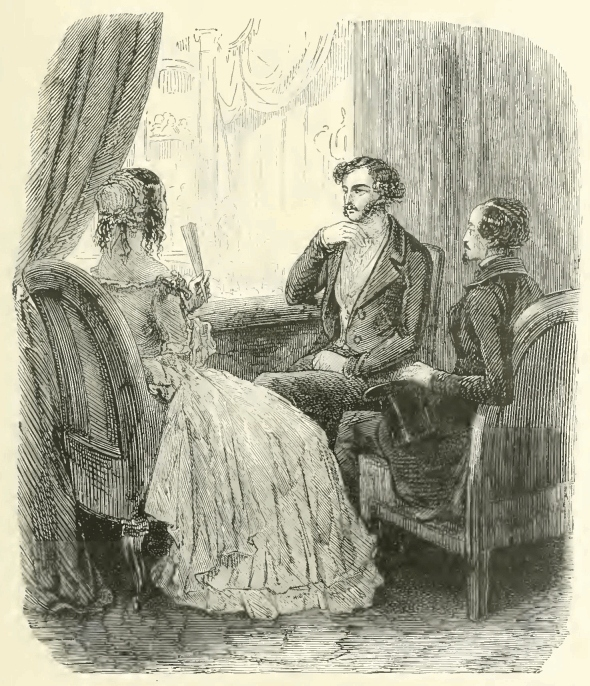
\includegraphics[width=\textwidth]{20181m.jpg}
\end{figure}

This precaution taken, they went to the theatre, and installed
themselves in the count’s box. During the first act, the Countess G——
entered. Her first look was at the box where she had seen the count the
previous evening, so that she perceived Franz and Albert in the place
of the very person concerning whom she had expressed so strange an
opinion to Franz. Her opera-glass was so fixedly directed towards them,
that Franz saw it would be cruel not to satisfy her curiosity; and,
availing himself of one of the privileges of the spectators of the
Italian theatres, who use their boxes to hold receptions, the two
friends went to pay their respects to the countess. Scarcely had they
entered, when she motioned to Franz to assume the seat of honor.
Albert, in his turn, sat behind.

“Well,” said she, hardly giving Franz time to sit down, “it seems you
have nothing better to do than to make the acquaintance of this new
Lord Ruthven, and you are already the best friends in the world.”

“Without being so far advanced as that, my dear countess,” returned
Franz, “I cannot deny that we have abused his good nature all day.”

“All day?”

“Yes; this morning we breakfasted with him; we rode in his carriage all
day, and now we have taken possession of his box.”

“You know him, then?”

“Yes, and no.”

“How so?”

“It is a long story.”

“Tell it to me.”

“It would frighten you too much.”

“So much the more reason.”

“At least wait until the story has a conclusion.”

“Very well; I prefer complete histories; but tell me how you made his
acquaintance? Did anyone introduce you to him?”

“No; it was he who introduced himself to us.”

“When?”

“Last night, after we left you.”

“Through what medium?”

“The very prosaic one of our landlord.”

“He is staying, then, at the Hôtel de Londres with you?”

“Not only in the same hotel, but on the same floor.”

“What is his name; for, of course, you know?”

“The Count of Monte Cristo.”

“That is not a family name?”

“No, it is the name of the island he has purchased.”

“And he is a count?”

“A Tuscan count.”

“Well, we must put up with that,” said the countess, who was herself
from one of the oldest Venetian families. “What sort of a man is he?”

“Ask the Vicomte de Morcerf.”

“You hear, M. de Morcerf, I am referred to you,” said the countess.

“We should be very hard to please, madam,” returned Albert, “did we not
think him delightful. A friend of ten years’ standing could not have
done more for us, or with a more perfect courtesy.”

“Come,” observed the countess, smiling, “I see my vampire is only some
millionaire, who has taken the appearance of Lara in order to avoid
being confounded with M. de Rothschild; and you have seen her?”

“Her?”

\begin{figure}[ht]
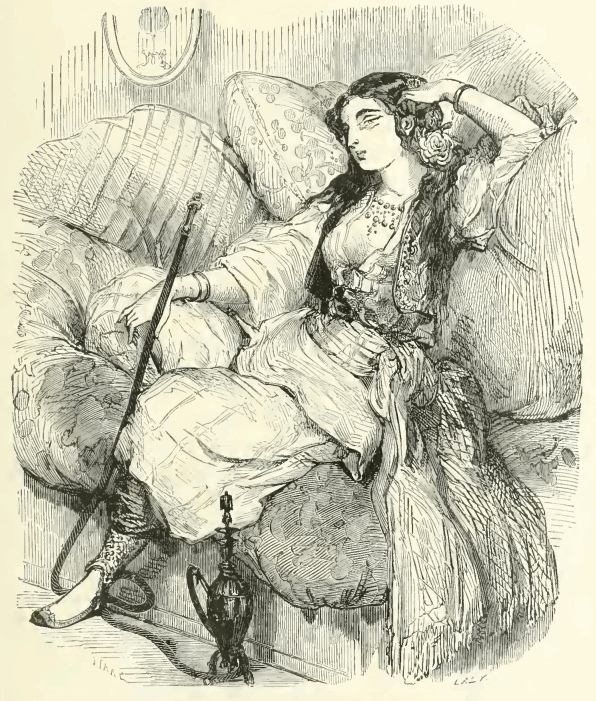
\includegraphics[width=\textwidth]{20183m.jpg}
\end{figure}

“The beautiful Greek of yesterday.”

“No; we heard, I think, the sound of her \textit{guzla}, but she remained
perfectly invisible.”

“When you say invisible,” interrupted Albert, “it is only to keep up
the mystery; for whom do you take the blue domino at the window with
the white curtains?”

“Where was this window with white hangings?” asked the countess.

“At the Rospoli Palace.”

“The count had three windows at the Rospoli Palace?”

“Yes. Did you pass through the Corso?”

“Yes.”

“Well, did you notice two windows hung with yellow damask, and one with
white damask with a red cross? Those were the count’s windows.”

“Why, he must be a nabob. Do you know what those three windows were
worth?”

“Two or three hundred Roman crowns?”

“Two or three thousand.”

“The deuce!”

“Does his island produce him such a revenue?”

“It does not bring him a bajocco.”

“Then why did he purchase it?”

“For a whim.”

“He is an original, then?”

“In reality,” observed Albert, “he seemed to me somewhat eccentric;
were he at Paris, and a frequenter of the theatres, I should say he was
a poor devil literally mad. This morning he made two or three exits
worthy of Didier or Anthony.”

At this moment a fresh visitor entered, and, according to custom, Franz
gave up his seat to him. This circumstance had, moreover, the effect of
changing the conversation; an hour afterwards the two friends returned
to their hotel.

Signor Pastrini had already set about procuring their disguises for the
morrow; and he assured them that they would be perfectly satisfied. The
next morning, at nine o’clock, he entered Franz’s room, followed by a
tailor, who had eight or ten Roman peasant costumes on his arm; they
selected two exactly alike, and charged the tailor to sew on each of
their hats about twenty yards of ribbon, and to procure them two of the
long silk sashes of different colors with which the lower orders
decorate themselves on fête days.

Albert was impatient to see how he looked in his new dress—a jacket and
breeches of blue velvet, silk stockings with clocks, shoes with
buckles, and a silk waistcoat. This picturesque attire set him off to
great advantage; and when he had bound the scarf around his waist, and
when his hat, placed coquettishly on one side, let fall on his shoulder
a stream of ribbons, Franz was forced to confess that costume has much
to do with the physical superiority we accord to certain nations. The
Turks used to be so picturesque with their long and flowing robes, but
are they not now hideous with their blue frocks buttoned up to the
chin, and their red caps, which make them look like a bottle of wine
with a red seal? Franz complimented Albert, who looked at himself in
the glass with an unequivocal smile of satisfaction. They were thus
engaged when the Count of Monte Cristo entered.

\begin{figure}[h]
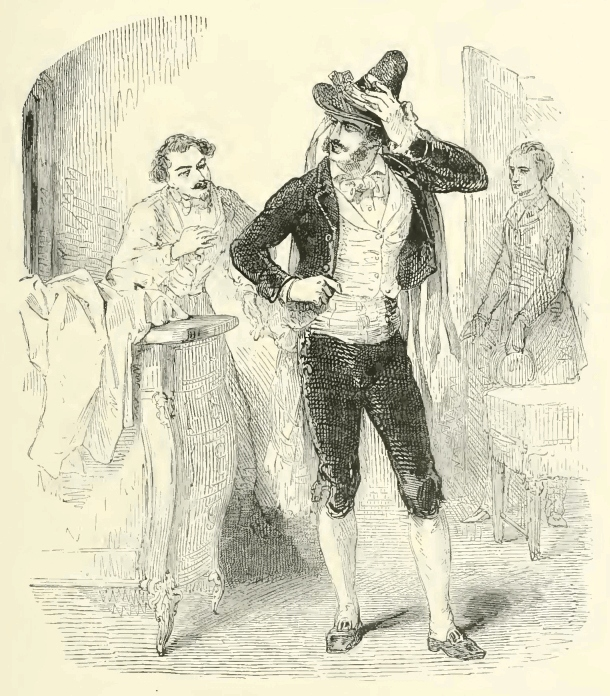
\includegraphics[width=\textwidth]{20185m.jpg}
\end{figure}

“Gentlemen,” said he, “although a companion is agreeable, perfect
freedom is sometimes still more agreeable. I come to say that today,
and for the remainder of the Carnival, I leave the carriage entirely at
your disposal. The host will tell you I have three or four more, so
that you will not inconvenience me in any way. Make use of it, I pray
you, for your pleasure or your business.”

The young men wished to decline, but they could find no good reason for
refusing an offer which was so agreeable to them. The Count of Monte
Cristo remained a quarter of an hour with them, conversing on all
subjects with the greatest ease. He was, as we have already said,
perfectly well acquainted with the literature of all countries. A
glance at the walls of his salon proved to Franz and Albert that he was
a connoisseur of pictures. A few words he let fall showed them that he
was no stranger to the sciences, and he seemed much occupied with
chemistry. The two friends did not venture to return the count the
breakfast he had given them; it would have been too absurd to offer him
in exchange for his excellent table the very inferior one of Signor
Pastrini. They told him so frankly, and he received their excuses with
the air of a man who appreciated their delicacy. Albert was charmed
with the count’s manners, and he was only prevented from recognizing
him for a perfect gentleman by reason of his varied knowledge.

The permission to do what he liked with the carriage pleased him above
all, for the fair peasants had appeared in a most elegant carriage the
preceding evening, and Albert was not sorry to be upon an equal footing
with them. At half-past one they descended, the coachman and footman
had put on their livery over their disguises, which gave them a more
ridiculous appearance than ever, and which gained them the applause of
Franz and Albert. Albert had fastened the faded bunch of violets to his
button-hole. At the first sound of the bell they hastened into the
Corso by the Via Vittoria.

At the second turn, a bunch of fresh violets, thrown from a carriage
filled with harlequins, indicated to Albert that, like himself and his
friend, the peasants had changed their costume also; and whether it was
the result of chance, or whether a similar feeling had possessed them
both, while he had donned their costume, they had assumed his.

Albert placed the fresh bouquet in his button-hole, but he kept the
faded one in his hand; and when he again met the calash, he raised it
to his lips, an action which seemed greatly to amuse not only the fair
lady who had thrown it, but her joyous companions also. The day was as
gay as the preceding one, perhaps even more animated and noisy; the
count appeared for an instant at his window, but when they again passed
he had disappeared. It is almost needless to say that the flirtation
between Albert and the fair peasant continued all day.

In the evening, on his return, Franz found a letter from the embassy,
informing him that he would have the honor of being received by his
holiness the next day. At each previous visit he had made to Rome, he
had solicited and obtained the same favor; and incited as much by a
religious feeling as by gratitude, he was unwilling to quit the capital
of the Christian world without laying his respectful homage at the feet
of one of St. Peter’s successors who has set the rare example of all
the virtues. He did not then think of the Carnival, for in spite of his
condescension and touching kindness, one cannot incline one’s self
without awe before the venerable and noble old man called Gregory XVI.

On his return from the Vatican, Franz carefully avoided the Corso; he
brought away with him a treasure of pious thoughts, to which the mad
gayety of the maskers would have been profanation.

At ten minutes past five Albert entered overjoyed. The harlequin had
reassumed her peasant’s costume, and as she passed she raised her mask.
She was charming. Franz congratulated Albert, who received his
congratulations with the air of a man conscious that they are merited.
He had recognized by certain unmistakable signs, that his fair
\textit{incognita} belonged to the aristocracy. He had made up his mind to
write to her the next day.

Franz remarked, while he gave these details, that Albert seemed to have
something to ask of him, but that he was unwilling to ask it. He
insisted upon it, declaring beforehand that he was willing to make any
sacrifice the other wished.

Albert let himself be pressed just as long as friendship required, and
then avowed to Franz that he would do him a great favor by allowing him
to occupy the carriage alone the next day. Albert attributed to Franz’s
absence the extreme kindness of the fair peasant in raising her mask.
Franz was not sufficiently egotistical to stop Albert in the middle of
an adventure that promised to prove so agreeable to his curiosity and
so flattering to his vanity. He felt assured that the perfect
indiscretion of his friend would duly inform him of all that happened;
and as, during three years that he had travelled all over Italy, a
similar piece of good fortune had never fallen to his share, Franz was
by no means sorry to learn how to act on such an occasion. He therefore
promised Albert that he would content himself the morrow with
witnessing the Carnival from the windows of the Rospoli Palace.

The next morning he saw Albert pass and repass, holding an enormous
bouquet, which he doubtless meant to make the bearer of his amorous
epistle. This belief was changed into certainty when Franz saw the
bouquet (conspicuous by a circle of white camellias) in the hand of a
charming harlequin dressed in rose-colored satin.

The evening was no longer joy, but delirium. Albert nothing doubted but
that the fair unknown would reply in the same manner. Franz anticipated
his wishes by saying that the noise fatigued him, and that he should
pass the next day in writing and looking over his journal. Albert was
not deceived, for the next evening Franz saw him enter triumphantly
shaking a folded paper which he held by one corner.

“Well,” said he, “was I mistaken?”

“She has answered you!” cried Franz.

“Read.”

This word was pronounced in a manner impossible to describe. Franz took
the letter, and read:

“Tuesday evening, at seven o’clock, descend from your carriage opposite
the Via dei Pontefici, and follow the Roman peasant who snatches your
torch from you. When you arrive at the first step of the church of San
Giacomo, be sure to fasten a knot of rose-colored ribbons to the
shoulder of your harlequin costume, in order that you may be
recognized. Until then you will not see me. —Constancy and Discretion.”

“Well,” asked he, when Franz had finished, “what do you think of that?”

“I think that the adventure is assuming a very agreeable appearance.”

“I think so, also,” replied Albert; “and I very much fear you will go
alone to the Duke of Bracciano’s ball.”

Franz and Albert had received that morning an invitation from the
celebrated Roman banker.

“Take care, Albert,” said Franz. “All the nobility of Rome will be
present, and if your fair \textit{incognita} belong to the higher class of
society, she must go there.”

“Whether she goes there or not, my opinion is still the same,” returned
Albert. “You have read the letter?”

“Yes.”

“You know how imperfectly the women of the \textit{mezzo cito} are educated in
Italy?” (This is the name of the lower class.)

“Yes.”

“Well, read the letter again. Look at the writing, and find if you can,
any blemish in the language or orthography.” The writing was, in
reality, charming, and the orthography irreproachable.

“You are born to good fortune,” said Franz, as he returned the letter.

“Laugh as much as you will,” replied Albert, “I am in love.”

“You alarm me,” cried Franz. “I see that I shall not only go alone to
the Duke of Bracciano’s, but also return to Florence alone.”

“If my unknown be as amiable as she is beautiful,” said Albert, “I
shall fix myself at Rome for six weeks, at least. I adore Rome, and I
have always had a great taste for archæology.”

\begin{figure}[ht]
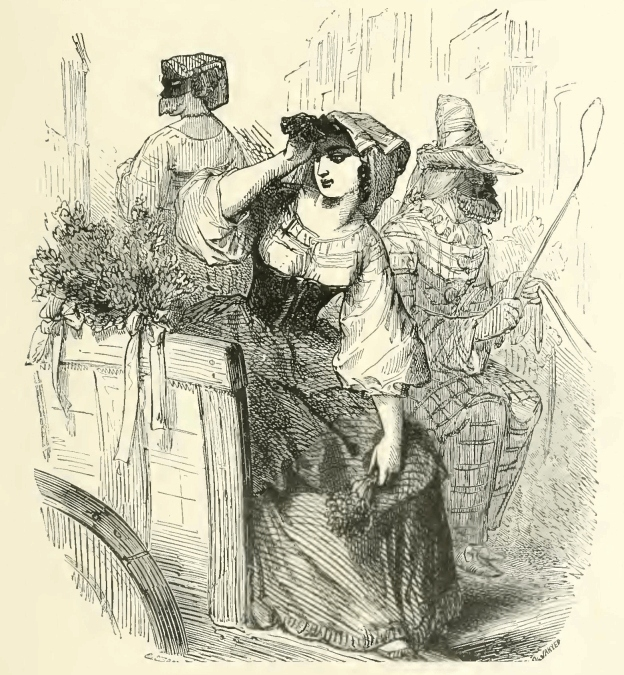
\includegraphics[width=\textwidth]{20189m.jpg}
\end{figure}

“Come, two or three more such adventures, and I do not despair of
seeing you a member of the Academy.”

Doubtless Albert was about to discuss seriously his right to the
academic chair when they were informed that dinner was ready. Albert’s
love had not taken away his appetite. He hastened with Franz to seat
himself, free to recommence the discussion after dinner. After dinner,
the Count of Monte Cristo was announced. They had not seen him for two
days. Signor Pastrini informed them that business had called him to
Civita Vecchia. He had started the previous evening, and had only
returned an hour since. He was charming. Whether he kept a watch over
himself, or whether by accident he did not sound the acrimonious chords
that in other circumstances had been touched, he was tonight like
everybody else.

The man was an enigma to Franz. The count must feel sure that Franz
recognized him; and yet he had not let fall a single word indicating
any previous acquaintance between them. On his side, however great
Franz’s desire was to allude to their former interview, the fear of
being disagreeable to the man who had loaded him and his friend with
kindness prevented him from mentioning it.

The count had learned that the two friends had sent to secure a box at
the Argentina Theatre, and were told they were all let. In consequence,
he brought them the key of his own—at least such was the apparent
motive of his visit. Franz and Albert made some difficulty, alleging
their fear of depriving him of it; but the count replied that, as he
was going to the Palli Theatre, the box at the Argentina Theatre would
be lost if they did not profit by it. This assurance determined the two
friends to accept it.

Franz had by degrees become accustomed to the count’s pallor, which had
so forcibly struck him at their first meeting. He could not refrain
from admiring the severe beauty of his features, the only defect, or
rather the principal quality of which was the pallor. Truly, a Byronic
hero! Franz could not, we will not say see him, but even think of him
without imagining his stern head upon Manfred’s shoulders, or beneath
Lara’s helmet. His forehead was marked with the line that indicates the
constant presence of bitter thoughts; he had the fiery eyes that seem
to penetrate to the very soul, and the haughty and disdainful upper lip
that gives to the words it utters a peculiar character that impresses
them on the minds of those to whom they are addressed.

The count was no longer young. He was at least forty; and yet it was
easy to understand that he was formed to rule the young men with whom
he associated at present. And, to complete his resemblance with the
fantastic heroes of the English poet, the count seemed to have the
power of fascination. Albert was constantly expatiating on their good
fortune in meeting such a man. Franz was less enthusiastic; but the
count exercised over him also the ascendency a strong mind always
acquires over a mind less domineering. He thought several times of the
project the count had of visiting Paris; and he had no doubt but that,
with his eccentric character, his characteristic face, and his colossal
fortune, he would produce a great effect there. And yet he did not wish
to be at Paris when the count was there.

The evening passed as evenings mostly pass at Italian theatres; that
is, not in listening to the music, but in paying visits and conversing.
The Countess G—— wished to revive the subject of the count, but Franz
announced he had something far newer to tell her, and, in spite of
Albert’s demonstrations of false modesty, he informed the countess of
the great event which had preoccupied them for the last three days. As
similar intrigues are not uncommon in Italy, if we may credit
travellers, the comtess did not manifest the least incredulity, but
congratulated Albert on his success. They promised, upon separating, to
meet at the Duke of Bracciano’s ball, to which all Rome was invited.

The heroine of the bouquet kept her word; she gave Albert no sign of
her existence the morrow or the day after.

At length Tuesday came, the last and most tumultuous day of the
Carnival. On Tuesday, the theatres open at ten o’clock in the morning,
as Lent begins after eight at night. On Tuesday, all those who through
want of money, time, or enthusiasm, have not been to see the Carnival
before, mingle in the gayety, and contribute to the noise and
excitement. From two o’clock till five Franz and Albert followed in the
\textit{fête}, exchanging handfuls of \textit{confetti} with the other carriages and
the pedestrians, who crowded amongst the horses’ feet and the carriage
wheels without a single accident, a single dispute, or a single fight.

The \textit{fêtes} are veritable pleasure days to the Italians. The author of
this history, who has resided five or six years in Italy, does not
recollect to have ever seen a ceremony interrupted by one of those
events so common in other countries. Albert was triumphant in his
harlequin costume. A knot of rose-colored ribbons fell from his
shoulder almost to the ground. In order that there might be no
confusion, Franz wore his peasant’s costume.

As the day advanced, the tumult became greater. There was not on the
pavement, in the carriages, at the windows, a single tongue that was
silent, a single arm that did not move. It was a human storm, made up
of a thunder of cries, and a hail of sweetmeats, flowers, eggs,
oranges, and nosegays.

At three o’clock the sound of fireworks, let off on the Piazza del
Popolo and the Piazza di Venezia (heard with difficulty amid the din
and confusion) announced that the races were about to begin.

The races, like the \textit{moccoli}, are one of the episodes peculiar to the
last days of the Carnival. At the sound of the fireworks the carriages
instantly broke ranks, and retired by the adjacent streets. All these
evolutions are executed with an inconceivable address and marvellous
rapidity, without the police interfering in the matter. The pedestrians
ranged themselves against the walls; then the trampling of horses and
the clashing of steel were heard. A detachment of carbineers, fifteen
abreast, galloped up the Corso in order to clear it for the \textit{barberi}.
When the detachment arrived at the Piazza di Venezia, a second volley
of fireworks was discharged, to announce that the street was clear.

Almost instantly, in the midst of a tremendous and general outcry,
seven or eight horses, excited by the shouts of three hundred thousand
spectators, passed by like lightning. Then the Castle of Saint Angelo
fired three cannon to indicate that number three had won.

Immediately, without any other signal, the carriages moved on, flowing
on towards the Corso, down all the streets, like torrents pent up for a
while, which again flow into the parent river; and the immense stream
again continued its course between its two granite banks.

A new source of noise and movement was added to the crowd. The sellers
of \textit{moccoletti} entered on the scene. The \textit{moccoli}, or \textit{moccoletti},
are candles which vary in size from the pascal taper to the rushlight,
and which give to each actor in the great final scene of the Carnival
two very serious problems to grapple with,—first, how to keep his own
\textit{moccoletto} alight; and secondly, how to extinguish the \textit{moccoletti}
of others. The \textit{moccoletto} is like life: man has found but one means
of transmitting it, and that one comes from God. But he has discovered
a thousand means of taking it away, and the devil has somewhat aided
him. The \textit{moccoletto} is kindled by approaching it to a light. But who
can describe the thousand means of extinguishing the \textit{moccoletto}?—the
gigantic bellows, the monstrous extinguishers, the superhuman fans.
Everyone hastened to purchase \textit{moccoletti}—Franz and Albert among the
rest.

The night was rapidly approaching; and already, at the cry of
“\textit{Moccoletti}!” repeated by the shrill voices of a thousand vendors,
two or three stars began to burn among the crowd. It was a signal. At
the end of ten minutes fifty thousand lights glittered, descending from
the Palazzo di Venezia to the Piazza del Popolo, and mounting from the
Piazza del Popolo to the Palazzo di Venezia. It seemed like the \textit{fête}
of Jack-o’-lanterns.

It is impossible to form any idea of it without having seen it. Suppose
that all the stars had descended from the sky and mingled in a wild
dance on the face of the earth; the whole accompanied by cries that
were never heard in any other part of the world. The \textit{facchino} follows
the prince, the Transteverin the citizen, everyone blowing,
extinguishing, relighting. Had old Æolus appeared at this moment, he
would have been proclaimed king of the \textit{moccoli}, and Aquilo the
heir-presumptive to the throne.

This battle of folly and flame continued for two hours; the Corso was
light as day; the features of the spectators on the third and fourth
stories were visible.

Every five minutes Albert took out his watch; at length it pointed to
seven. The two friends were in the Via dei Pontefici. Albert sprang
out, bearing his \textit{moccoletto} in his hand. Two or three masks strove to
knock his \textit{moccoletto} out of his hand; but Albert, a first-rate
pugilist, sent them rolling in the street, one after the other, and
continued his course towards the church of San Giacomo.

The steps were crowded with masks, who strove to snatch each other’s
torches. Franz followed Albert with his eyes, and saw him mount the
first step.

Instantly a mask, wearing the well-known costume of a peasant woman,
snatched his \textit{moccoletto} from him without his offering any resistance.
Franz was too far off to hear what they said; but, without doubt,
nothing hostile passed, for he saw Albert disappear arm-in-arm with the
peasant girl. He watched them pass through the crowd for some time, but
at length he lost sight of them in the Via Macello.

Suddenly the bell that gives the signal for the end of the Carnival
sounded, and at the same instant all the \textit{moccoletti} were extinguished
as if by enchantment. It seemed as though one immense blast of the wind
had extinguished everyone.

Franz found himself in utter darkness. No sound was audible save that
of the carriages that were carrying the maskers home; nothing was
visible save a few lights that burnt behind the windows.

The Carnival was over.

\begin{figure}[ht]
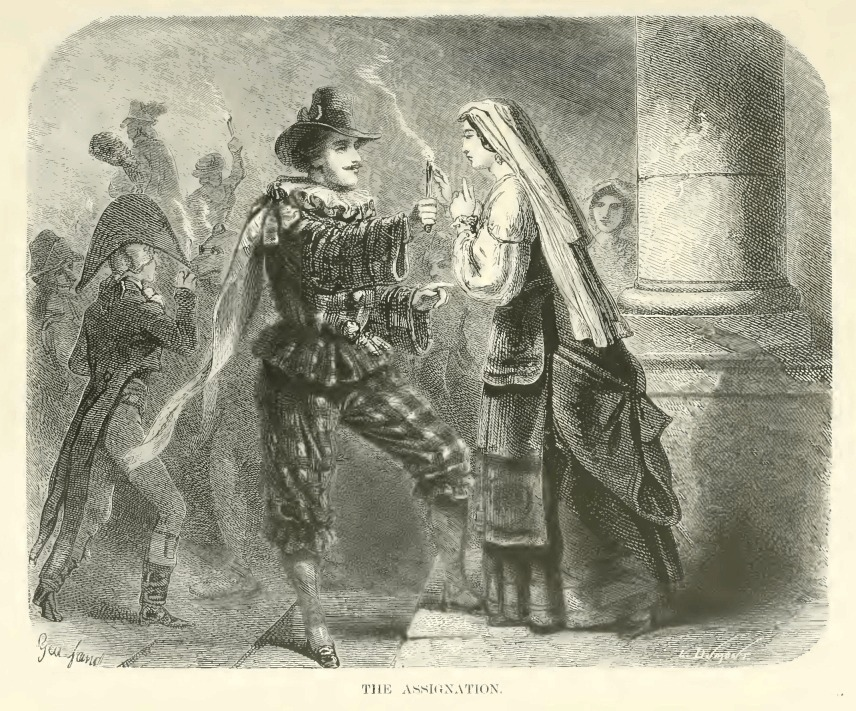
\includegraphics[width=\textwidth]{20193m.jpg}
\end{figure}
